\documentclass[../main.tex]{subfiles}

\begin{document}

\section{Configuración y compilación de Linux}

En este apartado se va a detallar el proceso de configuración y compilación del kernel Linux utilizado en prácticas para habilitar aquellos tracepoints del código que se deseaba utilizar para el trabajo.

También se van a comentar brevemente los modelos de expulsión configurados en cada una de las compilaciones realizadas.

%----------------------------------------------------------------------------------
\subsection{Obtención y preparación de los fuentes}

Primero, se han obtenido los fuentes del kernel del directorio de la asignatura en Hendrix \cite{fuentes-Linux}. Éstos cuentan ya con el \it{patch RT} aplicado, por lo que se puede pasar a preparar la compilación directamente:

\begin{codigo}{bash}
# Descomprimir el kernel
tar xJf kernel-rt.xz

# Preparar fuentes
cd kernel-rt/kernel
make ARCH=arm clean
mkdir rootfs
\end{codigo}

Tras ello, se ejecuta \it{make menuconfig} para poder llevar a cabo la configuración del kernel mediante un menú \it{ncurses} en lugar de editar directamente las variables del fichero de texto \it{.config}:

\begin{codigo}{bash}
# Abrir menú ncurses para la configuración
make ARCH=arm menuconfig
\end{codigo}

En los siguientes apartados se trata la configuración, usando dicho menú, del modelo de expulsión y los tracers que durante la compilación se quieren incluir.

%----------------------------------------------------------------------------------
\subsection{Modelo de expulsión}

Para elegir el modelo de expulsión del kernel se debe navegar a la sección \it{Kernel Features > Preemption Model} desde el menú principal. En ella, al haber aplicado el \it{patch RT}, se pueden ver las opciones siguientes:

\begin{figure}[htp]
    \centering
    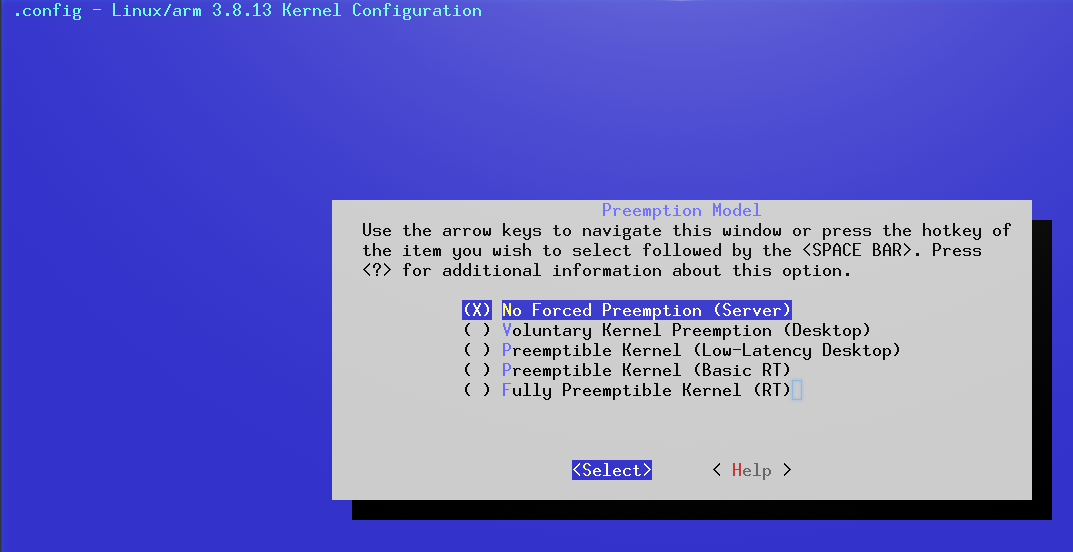
\includegraphics[width=15cm]{imagenes/capturas/Linux-make-menuconfig-Preemtion-model.png}
    \caption{Captura de la configuración establecida en menuconfig}
\end{figure}

Para el trabajo se van a utilizar los modelos \it{no forced preemption} y \it{full preemption}.

\it{No forced preemption} es el modelo de expulsión original de UNIX, y se utiliza especialmente para servidores. En él los \it{KCP}s en contexto de interrupción no se pueden bloquear, ya que no son planificables.

Por otra parte, \it{full preemption} es el modelo de expulsión pensado para tiempo real en Linux. En él todos los \it{KCP}s, incluidos los que se ejecutan en contexto de interrupción, son planificables. Entre otras modificaciones, aplicarlo supone que todos los \it{spinlocks} del kernel se convierten en semáforos, por lo que la espera activa en caso de bloqueo se convierte en una invocación directa al planificador. Con esa y otras medidas se busca maximizar el número de expulsiones que se realizan.

Dado que solo se puede configurar un modelo de expulsión, se han realizado dos compilaciones del kernel en las que solo se ha cambiado esta opción, dejando todas las que se comentan a continuación de igual forma.

%----------------------------------------------------------------------------------
\subsection{Tracers}

Para elegir llegar a la sección de configuración de los tracers hay que navegar a la sección \it{Kernel Hacking > Tracers} desde el menú principal.

Para la realización del trabajo se han seleccionado los tracers siguientes: \it{Kernel Function Tracer}, \it{Interrupts-off Latency Tracer}, \it{Scheduling Latency Tracer}, \it{Scheduling Latency Histogram} y \it{Trace syscalls}. Además, se han dejado marcadas aquellas opciones que se señalaban automáticamente al elegir las mencionadas. Así, las opciones del menú de configuración correspondiente a los tracers quedaba de la siguiente manera:

\begin{figure}[htp]
    \centering
    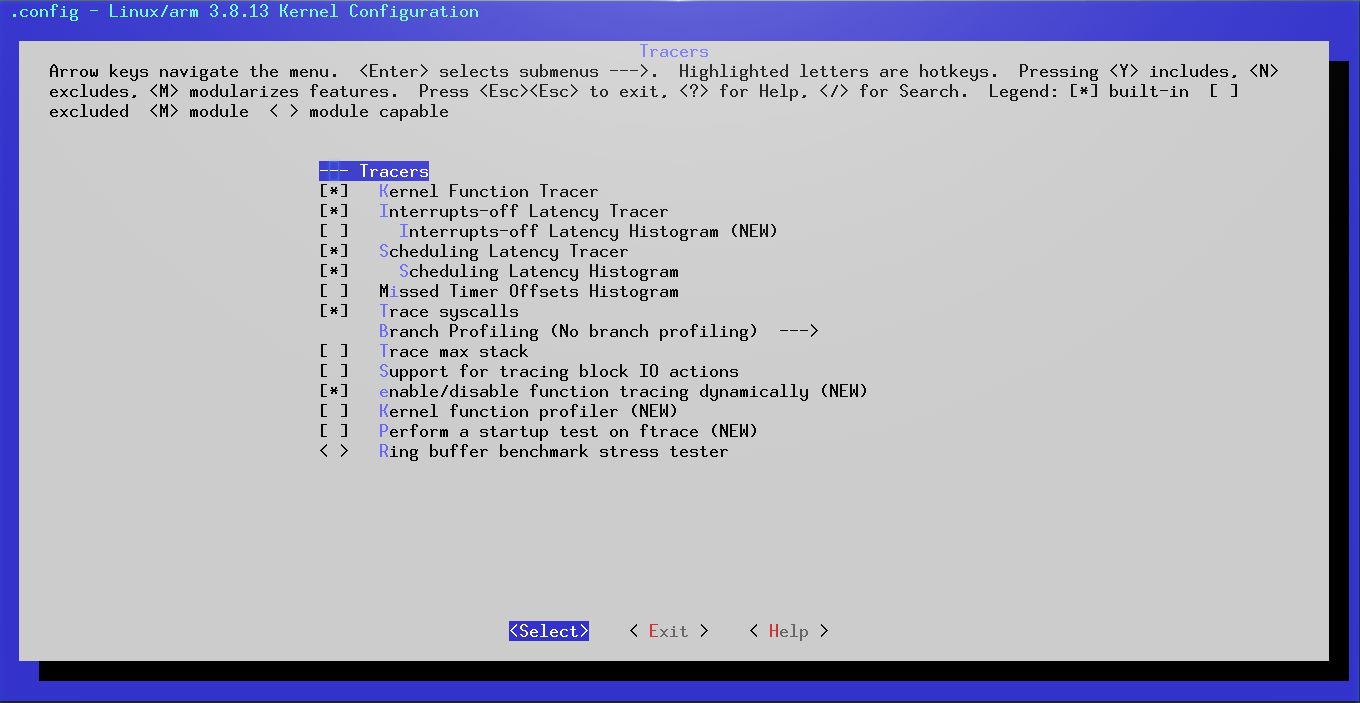
\includegraphics[width=15cm]{imagenes/capturas/Linux-make-menuconfig-tracers.png}
    \caption{Captura de la configuración establecida en menuconfig}
\end{figure}

Cabe destacar que la opción de elegir algunos tracers es dependiente del modelo de expulsión que se haya configurado; por ejemplo, el tracer \it{Preemption-off Latency Tracer} solo aparece cuando se ha configurado antes el modelo de expulsión como \it{Fully Preemptible Kernel}.

%----------------------------------------------------------------------------------
\subsection{Compilación}

Una vez realizada la configuración deseada, se procede a compilar el kernel, y se hace de manera análoga a como se hizo en la práctica tres de la asignatura:

\begin{codigo}{bash}
# Compilación del núcleo
export CC="/usr/local/linaro/gcc/bin/arm-linux-gnueabihf-"
make ARCH=arm CROSS_COMPILE=${CC} uImage dtbs
make ARCH=arm CROSS_COMPILE=${CC} modules
make ARCH=arm CROSS_COMPILE=${CC} INSTALL_MOD_PATH=${PWD}/rootfs modules_install
make ARCH=arm CROSS_COMPILE=${CC} uImage-dtb.am335x-bone
\end{codigo}

Este proceso se ha llevado a cabo para las dos configuraciones correspondientes a los distintos modelos de expulsión que se querían probar, dando como resultado dos kernels llamados \it{zImage\_ftrace\_FPK} y \it{zImage\_ftrace\_NFP}, siendo las letras del final las siglas del modelo de expulsión con el que se configuró la compilación.

\end{document}